\subsection{Image Builder} \label{subsection:eval_image_builder}

This subsection highlights how different variable configurations impact the total project, especially its image build times, which make up a significant part of it.

Figure \ref{fig:eval_3_cpu_and_mem} depicts the CPU and memory utilization of experiment (3).
Compared to (1), a project now only takes approximately eight minutes, and the FL-actors' build times shrunk from six to two and a half minutes.
The use of development base images leads to even greater acceleration when the underlying dependency structure of the ML repository is larger.
The base images do not apply to the trained model build because each trained model is unique.
The stage durations graph \ref{fig:eval_3_simplest_stage_durations} of experiment (3) highlights this acceleration.
All other metrics, such as net-IO, disk space, memory, or results, stay the same as in (1) because the only change is the reuse of base images.
Therefore, when people develop FLOps further, they should utilize this base-image functionality to speed up their progress.

Figure \ref{fig:eval_4_cpu_and_mem} shows the CPU and memory utilization of experiment (4).
It is immediately clear how much emulation slows down multi-platform projects compared to the base case.
A simple multi-platform project takes around 45 minutes.
The FL-actor image build stage takes 27 minutes, which is a 4.5-fold increase, and the multi-platform trained-model image build takes 13 minutes, which is a fivefold increase.
This stark difference is especially visible in Figure \ref{fig:eval_4_simplest_stage_durations}, which shows the stage durations of experiment (4).
Other metrics are also lightly affected by this change.
More disk space is needed. 
Experiment (4) uses up 17.5 GB instead of 14 GB due to the extra image layers.
This increase also influences the net-IO where (4) requires sending out 12 GB and receives 10 GB instead of (1)'s 9 GB and 5.5 GB.
In addition, the net-IO accumulated more traffic over the longer project run-time.
In conclusion, these findings prove that FLOps supports working multi-platform images.
However, this approach significantly increases build times when run on single machines instead of dedicated build machines with matching native architectures.

\begin{figure}[H]
    \begin{adjustwidth}{-0.2\paperwidth}{-0.2\paperwidth}
        \centering
        % 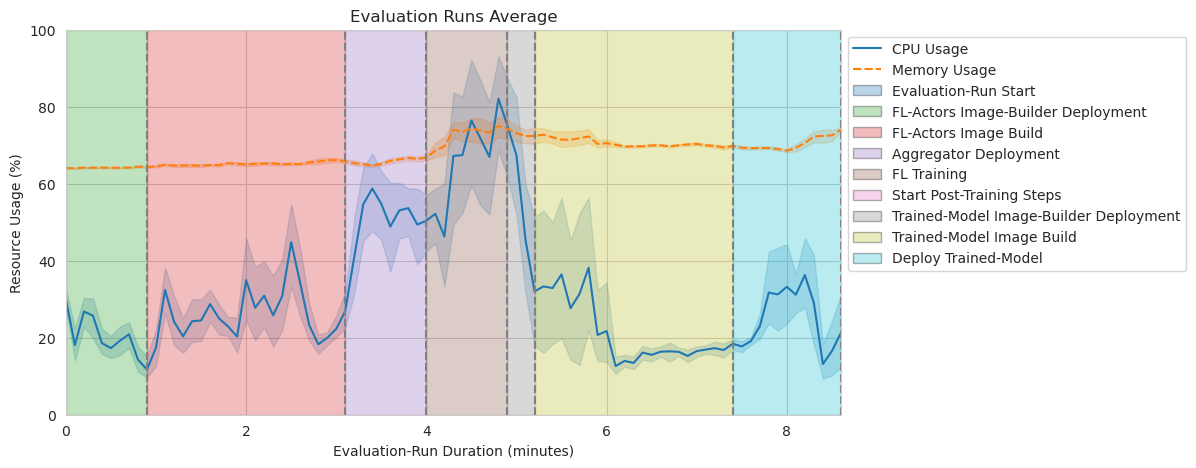
\includegraphics[width=0.90\paperwidth]{eval_3_simple_baseimages_cpu_and_mem.png}
        \includegraphics[width=0.90\paperwidth]{evaluations/experiment_3/cpu_mem.pdf}
        \caption{Experiment 3: CPU \& Memory Utilization}
        \label{fig:eval_3_cpu_and_mem}
    \end{adjustwidth}
\end{figure}

\begin{figure}[H]
    \begin{adjustwidth}{-0.2\paperwidth}{-0.2\paperwidth}
        \centering
        % 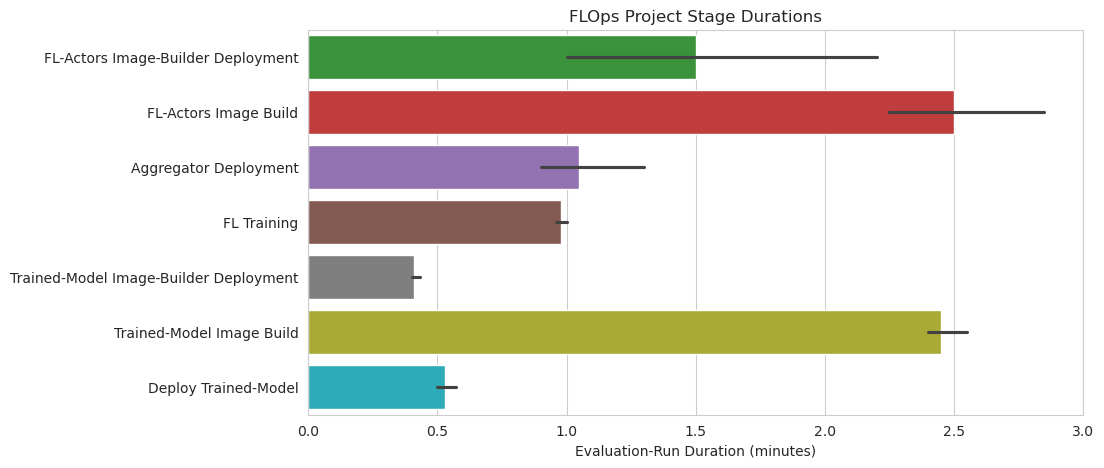
\includegraphics[width=0.95\textwidth]{eval_3_simple_baseimages_stage_durations.png}
        % \includegraphics[width=0.95\textwidth]{evaluations/experiment_3/stage_durations.pdf}
        \includegraphics[width=0.90\paperwidth]{evaluations/experiment_3/stage_durations.pdf}
        \caption{Experiment 3: Stage Durations}
        \label{fig:eval_3_simplest_stage_durations}
    \end{adjustwidth}
\end{figure}


\begin{figure}[H]
    \begin{adjustwidth}{-0.2\paperwidth}{-0.2\paperwidth}
        \centering
        % 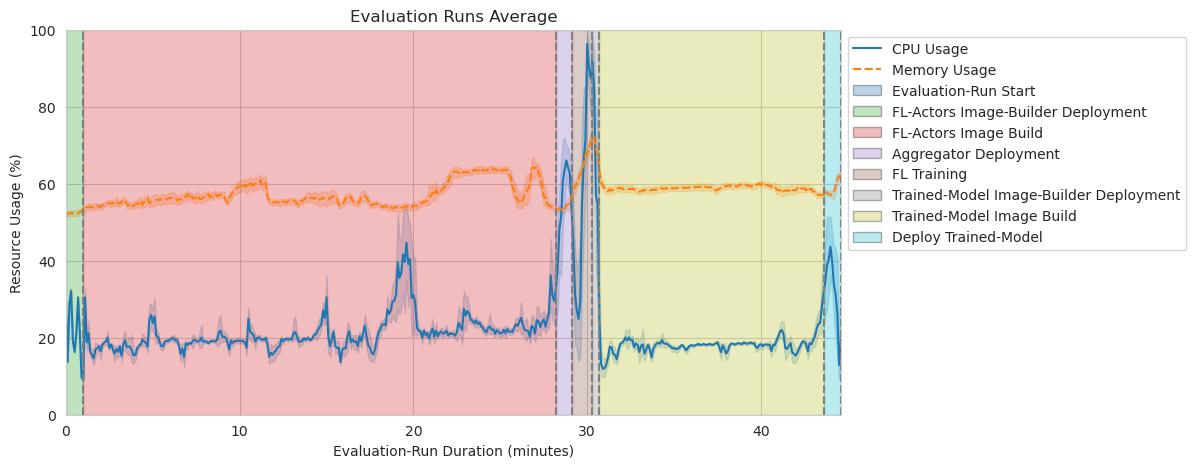
\includegraphics[width=0.90\paperwidth]{eval_4_simple_multiplatform_cpu_and_mem.png}
        \includegraphics[width=0.90\paperwidth]{evaluations/experiment_4/cpu_mem.pdf}
        \caption{Experiment 4: CPU \& Memory Utilization}
        \label{fig:eval_4_cpu_and_mem}
    \end{adjustwidth}
\end{figure}

\begin{figure}[H]
    \begin{adjustwidth}{-0.2\paperwidth}{-0.2\paperwidth}
        \centering
        % 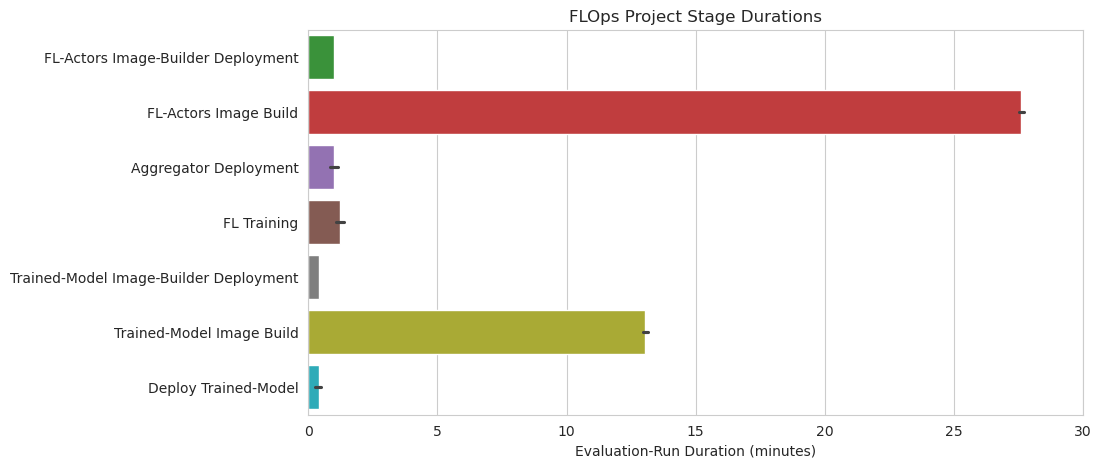
\includegraphics[width=0.95\textwidth]{eval_4_simple_multiplatform_stage_durations.png}
        \includegraphics[width=0.90\paperwidth]{evaluations/experiment_4/stage_durations.pdf}
        \caption{Experiment 4: Stage Durations}
        \label{fig:eval_4_simplest_stage_durations}
    \end{adjustwidth}
\end{figure}
